
% to choose your degree
% please un-comment just one of the following
\documentclass[bsc,frontabs,twoside,singlespacing,parskip,deptreport]{infthesis}     % for BSc, BEng etc.
% \documentclass[minf,frontabs,twoside,singlespacing,parskip,deptreport]{infthesis}  % for MInf

\usepackage[utf8]{inputenc}
\usepackage{epigraph}
\usepackage{graphicx} %Added by Songbo



\begin{document}

\title{Building Coherent Open-domain Dialogue Systems Using Neural Networks}

\author{Songbo Hu}

% to choose your course
% please un-comment just one of the following
\course{Artificial Intelligence and Computer Science}
%\course{Artificial Intelligence and Software Engineering}
%\course{Artificial Intelligence and Mathematics}
%\course{Artificial Intelligence and Psychology }   
%\course{Artificial Intelligence with Psychology }   
%\course{Linguistics and Artificial Intelligence}    
%\course{Computer Science}
%\course{Software Engineering}
%\course{Computer Science and Electronics}    
%\course{Electronics and Software Engineering}    
%\course{Computer Science and Management Science}    
%\course{Computer Science and Mathematics}
%\course{Computer Science and Physics}  
%\course{Computer Science and Statistics}    

% to choose your report type
% please un-comment just one of the following
%\project{Undergraduate Dissertation} % CS&E, E&SE, AI&L
%\project{Undergraduate Thesis} % AI%Psy
\project{4th Year Project Report}

\date{\today}

\abstract{
Add abstract later.
}

\maketitle

\section*{Acknowledgements}
Acknowledgements go here. 

\tableofcontents

%\pagenumbering{arabic}


\chapter{Introduction}

\epigraph{Sorry, I'm still not sure about that.}{\textit{Siri 2020}}

A dialogue system is a conversational agent that can converse with humans in natural language. It can help us solve many tedious tasks effectively or bring entertainment value to our daily life. Recent advances in dialogue systems (such as virtual assistants) enable us to engage in natural conversational interactions with computers. It substantially increases the accessibility of state of the art technologies to people with diverse backgrounds. And for those with impairments, it could transform their daily living into a journey toward capability instead of disability.

Since Alan Turing published his landmark work in 1950\cite{turing1950computing}, the intelligence level of a machine is described as how well the machine is able to fool a human into believing that it, the machine, is a human based on its text responses. If the human evaluator cannot tell the difference between the machine from a human, the machine is said to have passed the Turing test, which signifies a high level of intelligence of an AI. It has been the goal for the development of dialogue systems for decades and there are various attempts have been proposed to pass the test. Recently, advances in neural network based language models enable us to learn entire dialogue models directly from conversational data. But we are still far from passing the test. Most of the previous systems have failed to model the longer prior context of the conversation adequately, thereby creating a situation where extended dialogues rapidly become incoherent and unnatural sounding, with repetition being a key problem. Like I mentioned above, Siri fails to model elided constructions and produces repetitive responses. It is a problem which need to be adequately solved before our agents could move forward and pass the Turing test.

In this section, we will briefly review the recent development of dialogue systems. Specifically, we will discuss two types of dialogue systems: the chit-chat system and goal oriented dialogue system, particularly current spoken dialogue system (hereafter SDS). We will discuss their architectures, pros and cons, and why their main limitations to pass the Turing test. The majority of this thesis is about how to create an environment for neural models to learn the linguistic patterns within coherent extended dialogues and how to integrate this model into the existing dialogue systems to enable them utilising useful linguistic information and produce coherent responses.

\section {A Brief Review of Existing Dialogue Systems}

\subsection{The Chit-chat Dialogue System}

The chit-chat-oriented dialogue systems are usually called chatbots. These systems are designed and implemented with the goal carrying extended conversations with the goal of mimicking the unstructured conversations or ‘chats’ characteristic of informal human-human interaction. They are mainly aiming to provide entertainment value to our daily life. Existing chatbots majorly fall into the following three subcategories: the rule-based systems, the corpus-based systems, as will be discussed in order below.

\subsubsection*{The rule-based systems}

Instead of letting machines learning the conversation strategy from human behaviours, we could ask humans to encode these human intelligence directly as rules. Then dialogue agents could use these rules to generate dialogue utterances effectively. Normally, a message input will be processed by a set of carefully pre-defined rules e.g., a key-word look-up dictionary, if-else conditions, or more sophisticated machine learning classifiers. After rule conditions are evaluated, relevant actions will be executed, such as outputting an utterance in storage, manipulating the input message or selecting some related historical contexts.

\begin{figure}[h]
    \centering
    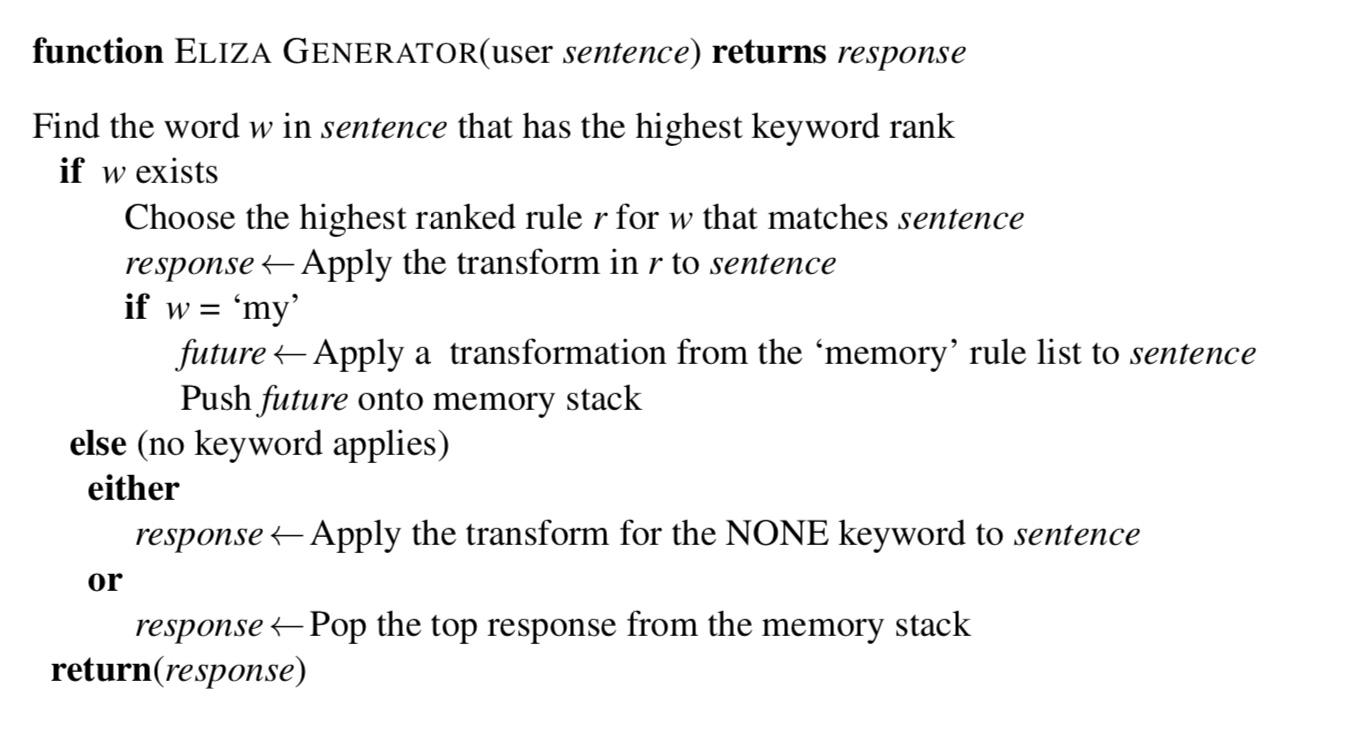
\includegraphics[width=0.9\textwidth]{elizarule.jpeg}
    \caption{A simplified sketch of the ELIZA algorithm.}
    \label{fig:elizarule}
\end{figure}

One of the epoch-making rule-based dialogue systems in history is ELIZA\cite{weizenbaum1966eliza}. ELIZA operates by first searching a keyword existing in the input text from a real human based on a hand-crafted keyword dictionary. If a keyword is found, a rule is applied to manipulate and transform the user’s original input and forwarded back to the user. Otherwise, ELIZA responded either with a generic response or copying one sentence from the dialogue history. There are many extensions of ELIZA, for example, PARRY\cite{parkinson1977conversational} and ALICE\cite{wallace1995artificial}. PARRY,, which simulated a patient with schizophrenia, relies on global variables to keep track of the emotional state, as opposed to ELIZA where responses are generated only based on the previous sentence. Artificial Intelligence Markup Language(AIML), which is the basis of ALICE, provides an effect tool to write sophisticated conversations logic in a machine-readable format.

ELIZA-style systems are recognized as an important milestone in developing modern dialogue systems. Even nowadays, with the rapid development of fancy neural network architecture and increasing number of conversational corpora, these rule-based dialogue systems could be a very strong baseline. On the other hand, their drawbacks are obvious: Rule-based systems predominantly rely on the set of pre-defined rules and these rules have to be carefully designed and implemented. Building a sophisticated rule-based system is very expensive because the number of these rules skyrockets. Rule-based systems do not have the ability to understand human languages, nor do they know how to generate meaningful natural language utterances. Consequently, they are very brittle and only able to conduct very superficial conversations.

\subsubsection*{The corpus-based systems}

Coding conversations logic manually is astronomically expensive and infeasible for many applications. Many researchers suggest to utilize large scale human conversational data and use statistic techniques to teach machines how to talk.

 This idea was firstly developed by Ritter et al. (cited in Jurafsky and Martin\cite{jurafsky2019speech}) using phrase-based machine translation to translate a user turn to a system response. In 2015, transduction models for response generation were modelled instead using encoder-decoder (seq2seq) models
 
 
 (Shang et al., 2015, Vinyals and Le 2015, and Sordoni et al. 2015 cited in Jurafsky and Martin, 2018). However, the simple seq2seq generation architecture is unable to model the prior context of the conversation. Serban et al (2016) suggests a hierarchical (HRED) model that summarizes information over multiple prior turns. This model consists of two RNNs stacked on top of each other: one is a sentence-level RNN which encodes each utterance into a fixed length vector, while a conversation-level RNN takes as input each utterance vector and outputs a vector that summarizes the conversation so far. The vector is mapped back to text using a recurrent decoder. This gives a way for the previous information to be passed to future turns as hidden states (Lowe et al. 2017).



\subsection{The Goal-oriented Dialogue system}




\section {Challenges}



\section {Thesis Outline}

\begin{itemize}
\item
The title page  in the format used above.
\item
An optional acknowledgements page.
\item
The table of contents.
\item
The report text divided into chapters as appropriate.
\item
The bibliography.
\end{itemize}

Commands for generating the title page appear in the skeleton file and
are self explanatory.
The file also includes commands to choose your report type (project
report, thesis or dissertation) and degree.
These will be placed in the appropriate place in the title page. 

The default behaviour of the documentclass is to produce documents typeset in
12 point.  Regardless of the formatting system you use, 
it is recommended that you submit your thesis printed (or copied) 
double sided.

The report should be printed single-spaced.
It should be 30 to 60 pages long, and preferably no shorter than 20 pages.
Appendices are in addition to this and you should place detail
here which may be too much or not strictly necessary when reading the relevant section.


Divide your chapters into sub-parts as appropriate.








\chapter{Background}

Of course
you may want to use several chapters and much more text than here.

\chapter{Extended Dialogues Grounded on Knowledge Graph: A Corpus}

\chapter{Statistical Analysis}

\chapter{Modelling Coherent Dialogues with Neural Network}

\chapter{Towards Building Coherent Open-domain Dialogue Systems}

\chapter{Discussion}

\chapter{Conclusion and Future Work}


\section{Citations}


Note that citations 
(like \cite{P1} or \cite{P2})
can be generated using {\tt BibTeX} or by using the
{\tt thebibliography} environment. This makes sure that the
table of contents includes an entry for the bibliography.
Of course you may use any other method as well.

\section{Options}

There are various documentclass options, see the documentation.  Here we are
using an option ({\tt bsc} or {\tt minf}) to choose the degree type, plus:
\begin{itemize}
\item {\tt frontabs} (recommended) to put the abstract on the front page;
\item {\tt twoside} (recommended) to format for two-sided printing, with
  each chapter starting on a right-hand page;
\item {\tt singlespacing} (required) for single-spaced formating; and
\item {\tt parskip} (a matter of taste) which alters the paragraph formatting so that
paragraphs are separated by a vertical space, and there is no
indentation at the start of each paragraph.
\end{itemize}





% use the following and \cite{} as above if you use BibTeX
% otherwise generate bibtem entries
\bibliographystyle{plain}
\bibliography{mybibfile}

\end{document}
